\chapter{Arduino}
\label{sec:arduino}
Arduino is an open source platform, which makes the designing of an interactive or general electronics system easier. This is also why the Arduino platform is used at school for learning about electronics. It is developed by the students David Cuartielles, Gianluca Martino, Tom Igoe, David Mellis, and Massimo Banzi at the Interaction Design Institute Ivrea in Italy\cite{makingofarduino}.

Arduino boards have a set op input and output ports enabling it to read from a sensor, or a button and then maybe activate a motor or an LED light. How the arduino handles or reacts to input is up to the designer which can program the Arduino board using the Arduino IDE.

"Arduino" covers a huge platform with a lot of different boards greatly varying in size, from Arduino Nano up to Arduino Mega. One of the more popular Arduino boards is the Arduino Uno which is somewhere in the middle of boards, considering size and power.

In the following subsections, the Uno and Mega, which will be used in this project, will be described.

\section{Arduino Uno}
One of the most common boards is the Arduino Uno \ref{fig:arduinouno}, which is based on the ATmega328 microcontroller. It has 14 digital input/output pins, and 6 analog inputs for connecting the different components. Considering specifications, which is shown on \ref{tab:unospec}, the Uno is limited on its resources. Therefore it is needed to limit both program- and datasize, and also the amount of complex tasks.
\begin{figure}[h!]
\centering
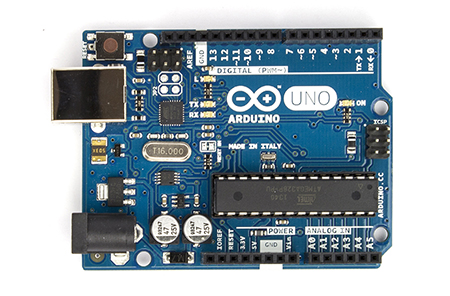
\includegraphics[width=0.5\textwidth]{chapters/analysis/figs/ArduinoUno.jpg}
\caption{Arduino Uno board\cite{arduinointroduction}.}
\label{fig:arduinouno}
\end{figure}

\begin{table}
\begin{tabular}{| l | l |}
\hline
Microcontroller & ATmega328\\
Operating Voltage & 5V\\
Input Voltage (recommended) & 7-12V\\
Input Voltage (limits) & 6-20V\\
Digital I/O Pins & 14 (of which 6 provide PWM output)\\
Analog Input Pins & 6\\
DC Current per I/O Pin & 40 mA\\
DC Current for 3.3V Pin & 50 mA\\
Flash Memory & 32 KB (ATmega328) of which 0.5 KB is used by bootloader\\
SRAM & 2 KB (ATmega328)\\
EEPROM & 1 KB (ATmega328)\\
Clock Speed & 16 MHz\\
\hline
\end{tabular}
\end{table}
\label{tab:unospec}
\section{Arduino Mega}
The Arduino Mega is a larger version of the Uno for some specifications. The Mega is larger on its memory and Pins, which makes it better for handling larger programs or amounts of data. Also a lot more components can be connected to the board. Since the clock speed is the same as the Uno, the Mega will not process data faster.

\begin{figure}[h!]
\centering
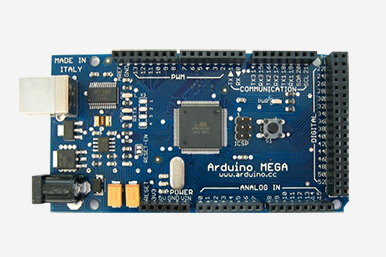
\includegraphics[width=0.5\textwidth]{chapters/analysis/figs/ArduinoMega.jpg}
\caption{Arduino Mega board\cite{arduinomega}.}
\label{fig:arduinomega}
\end{figure}

\begin{table}
\begin{tabular}{| l | l |}
\hline
Microcontroller & ATmega1280\\
Operating Voltage & 5V\\
Input Voltage (recommended) & 7-12V\\
Input Voltage (limits) & 6-20V\\
Digital I/O Pins & 54 (of which 15 provide PWM output)\\
Analog Input Pins & 16\\
DC Current per I/O Pin & 40 mA\\
DC Current for 3.3V Pin & 50 mA\\
Flash Memory & 128 KB of which 4 KB used by bootloader\\
SRAM & 8 KB\\
EEPROM & 4 KB\\
Clock Speed & 16 MHz\\
\hline
\end{tabular}
\end{table}
\label{tab:megaspec}